\documentclass[11pt]{report}

\usepackage{graphicx} % Add pictures to your document
\usepackage{listings}
\usepackage{float}
\usepackage{xcolor}
\usepackage{pgfplots}
\usepackage{sectsty}

\begin{document}

\title{\huge{\textbf{RCOM Lab2}} \\ Turma 3 // Grupo 3 \\ RCOM 2020/2021 \\ MIEIC FEUP}
\author{João de Jesus Costa \\ \texttt{up201806560} \and
	João Lucas Silva Martins \\ \texttt{up201806436}}
\date{\today{}}

\begin{figure}[b]
  \begin{center}
    
\includegraphics[width=0.6\textwidth]{feup_logo.png}
  \end{center}
\end{figure}
\maketitle{}

\tableofcontents{}
\newpage

\chapter{Summary}

This report documents the project that was developed for the curricular unit
of RCOM (FEUP). We implemented a simple FTP download application and configured
a computer network with three computers, a commercial router and switch.

\chapter{Introduction}

In the first part of this report, we'll focus on the FTP download application
and its architecture.\\
In the second part of this report, we'll focus on the network configuration
and analyze it.

\chapter{Part 1 - Download application}

\section{Architecture}

The application works linearly. We start by opening a socket to the given
server (on the standard FTP port: 21) and authenticate the user. This is
the \textbf{control socket}.\\
After the authentication process, we enter passive mode (with the PASV
command) and open a second socket to the server on the port replied on
the PASV command. This is the \textbf{data socket}.

Once we have this two sockets open, we just need to request the file
we want to the control socket and read it from the data socket. If any
of the steps described fails, the execution is aborted and the user is
informed of the error.

\section{Download steps}
\begin{enumerate}
\item Parse the url and authentication information
\item Resolve the hostname
\item Open control socket to server
\item Authenticate
\item Enter passive mode
\item Open data socket to server
\item Request file on control socket
\item Read file from the data socket
\end{enumerate}

\section{Report of a successful download}

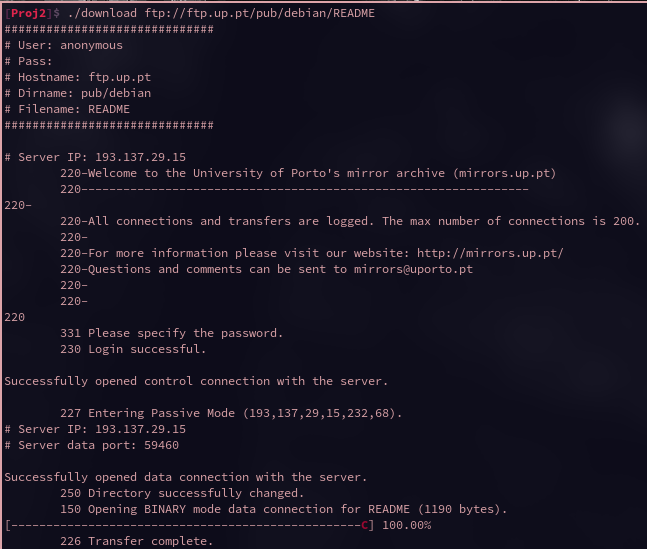
\includegraphics[width=1\textwidth]{images/download_report.png}

\chapter{Part 2 - Network configuration and analysis}

\section{Experience 1 - Configure an IP Network}

\subsection{Objectives}
Connect two hosts to a local network (switch) and enable communication between
them.

\subsection{Configuration commands}
\begin{lstlisting}
# on tux3
ifconfig eth0 172.16.60.1/24

# on tux4
ifconfig eth0 172.16.60.254/24
\end{lstlisting}

\paragraph{What are the ARP packets and what are they used for?}
ARP packets contain an IP address and are broadcast in the local network
(except to the source host). The host whose IP address is listed in the packet
sends a packet to the source host containing its MAC address. This way,
a host can find the MAC address of a host they only know the IP address of.

\paragraph{What are the MAC and IP addresses of ARP packets and why?}
ARP request packets contain the IP and MAC address of the sender host and the IP
address of the destination host. ARP reply packets include the destination
host's MAC address and are sent back to the source machine.\\
For example, \textbf{Tux3} sent an ARP packet asking who has the IP address
\textit{172.16.60.254}. The reply was sent by \textbf{Tux4} who had that IP address.

\paragraph{What packets does the ping command generate?}
The ping command generates ICMP ECHO\_REQUEST packet and expect
ICMP ECHO\_RESPONSE packet from a host or gateway.

\paragraph{What are the MAC and IP addresses of the ping packets?}
On the request ping packets, the IP and MAC addresses of the source correspond
to the source host's and the IP and MAC addresses of the destination correspond
to the destination host's. These switch places in the reply packet.\\
For example, \textbf{Tux3} sent a ping to the IP address \textit{172.16.60.254}
which corresponds to \textbf{Tux4}. The source IP and MAC addresses are
\textit{172.16.60.1} and \textit{00:21:5a:61:2d:df} respectively and the destination
IP and MAC addresses are \textit{172.16.60.254} and \textit{00:21:5a:5a:79:97}
on the request packet.

\paragraph{How to determine if a receiving Ethernet frame is ARP, IP, ICMP?}
We check the EtherType field on the Ethernet header of the MAC frame. The value is
\textbf{0x0800} for IPv4, \textbf{0x0806} for ARP and \textbf{0x86DD} for IPv6.\\
To check if the Ethernet frame contains an ICMP packet, we need to check the
protocol field of the IP packet header. The value is \textbf{1} for ICMP.

\paragraph{How to determine the length of a receiving frame?}
The EtherType field of the header of a Ethernet frame is two octets long and can
have two purposes. Values of less than or equal to 1500 indicate the size of the
payload in bytes. Values above 1536 indicate which protocol is encapsulated in
the payload of the frame. In this second case, the length of the frame can be
determined by determining the length of the encapsulated packet.

\paragraph{What is the loopback interface and why is it important?}
The loopback network specified by the IP protocol has the (IPv4) address
\textit{127.0.0.0/8}. On most IP implementations, any traffic sent to this network
is routed to the same computer. The most commonly used IP address for the
loopback interface is \textit{127.0.0.1} for IPv4 and \textit{::1} for IPv6.\\
This interface is useful to test and/or run client-server application/services
on the local machine.

\chapter{Conclusions}

\chapter{References}

\chapter{Annexes}

\end{document}
